\documentclass{beamer}
\usetheme{Boadilla}

\makeatother
\setbeamertemplate{footline}
{
    \leavevmode%
    \hbox{%
    \begin{beamercolorbox}[wd=.4\paperwidth,ht=2.25ex,dp=1ex,center]{author in head/foot}%
        \usebeamerfont{author in head/foot}\insertshortauthor
    \end{beamercolorbox}%
    \begin{beamercolorbox}[wd=.55\paperwidth,ht=2.25ex,dp=1ex,center]{title in head/foot}%
        \usebeamerfont{title in head/foot}\insertshorttitle
    \end{beamercolorbox}%
    \begin{beamercolorbox}[wd=.05\paperwidth,ht=2.25ex,dp=1ex,center]{date in head/foot}%
        \insertframenumber{}
    \end{beamercolorbox}}%
    \vskip0pt%
}
\makeatletter
\setbeamertemplate{navigation symbols}{}

\usepackage{lmodern}
\usepackage{amssymb,amsmath}
\renewcommand{\familydefault}{\sfdefault}

\DeclareMathOperator*{\argmax}{argmax}

\usepackage{mathtools}
\usepackage{graphicx}
\usepackage{threeparttable}
\usepackage{booktabs}
\usepackage{siunitx}
\sisetup{parse-numbers=false}

% \setlength{\OuterFrameSep}{-2pt}
% \makeatletter
% \preto{\@verbatim}{\topsep=-10pt \partopsep=-10pt }
% \makeatother

\title[Week 0:\ Course Overview]{Week 0:\ Course Overview}
\author[ResEcon 703:\ Advanced Econometrics]{ResEcon 703:\ Topics in Advanced Econometrics}
\date{Matt Woerman\\University of Massachusetts Amherst}

\begin{document}

{\setbeamertemplate{footline}{} 
\begin{frame}[noframenumbering]
    \titlepage
\end{frame}
}

\section{Agenda}
\begin{frame}\frametitle{Agenda}
    Today's topics
    \begin{itemize}
        \item \hyperlink{page.\getpagerefnumber{safety}}{Safety measures}
    	\item \hyperlink{page.\getpagerefnumber{introductions}}{Introductions}
        \item \hyperlink{page.\getpagerefnumber{information}}{Course information}
        \item \hyperlink{page.\getpagerefnumber{materials}}{Course materials}
        \item \hyperlink{page.\getpagerefnumber{grades}}{Grades and assignments}
    \end{itemize}
\end{frame}

\section{Safety Measures}
\label{safety}
\begin{frame}\frametitle{}
    \vfill
    \centering
    \begin{beamercolorbox}[center]{title}
        \Large Safety Measures
    \end{beamercolorbox}
    \vfill
\end{frame}

\begin{frame}\frametitle{University Guidelines}
    The university administration has instituted strict safety measures that will dictate the \emph{minimum} of what we will follow in this classroom
    \vspace{3ex}
    \begin{center}
        \href{https://www.umass.edu/coronavirus/}{\texttt{www.umass.edu/coronavirus}}
    \end{center}
\end{frame}

\begin{frame}\frametitle{Classroom Safety}
    As the semester begins, we will follow these classroom safety measures
    \begin{itemize}
        \item Everyone in the classroom must wear a mask
        \begin{itemize}
            \item A mask must cover your nose and mouth to be effective
        \end{itemize}
        \item Distance yourself from others if requested
        \begin{itemize}
            \item Six feet (or more) is a good benchmark, if possible
        \end{itemize}
        \item No eating in the classroom
        \item Anything else?
    \end{itemize}
    \vspace{3ex}
    Anyone not following these safety measures will be asked \emph{once} to correct the situation
    \begin{itemize}
        \item Not correcting the situation will result in expulsion from the classroom and a report to the Dean of Student Office
    \end{itemize}
\end{frame}

\begin{frame}\frametitle{Future Safety Measures}
    I will continually reevaluate these safety measures, as circumstances and university guidance evolve throughout the semester
    \begin{itemize}
        \item We will always follow---at a \emph{minimum}---university guidelines
    \end{itemize}
    \vspace{6ex}
    If you ever have any classroom safety concerns or have additional suggestions on how to ensure a safe learning environment, please let me know
\end{frame}

\section{Introductions}
\label{introductions}
\begin{frame}\frametitle{}
    \vfill
    \centering
    \begin{beamercolorbox}[center]{title}
        \Large Introductions
    \end{beamercolorbox}
    \vfill
\end{frame}

\begin{frame}\frametitle{My Info}
    Matt Woerman
    \begin{itemize}
        \item Assistant Professor, Resource Economics
    \end{itemize}
    \vspace{2ex}
    Contact info
    \begin{itemize}
        \item Email: \href{mailton:mwoerman@umass.edu}{\texttt{mwoerman@umass.edu}}
        \item Office hours: Tuesday, 1--3 pm, 218 Stockbridge Hall or Zoom
        \begin{itemize}
        	\item Sign up at: \href{https://calendly.com/mwoerman/officehours}{\texttt{calendly.com/mwoerman/officehours}} or \href{https://sites.google.com/site/mattwoerman/teaching}{\texttt{sites.google.com/site/mattwoerman/teaching}}
        \end{itemize}
    \end{itemize}
    \vspace{2ex}
    Best way to communicate with me
    \begin{itemize}
        \item ``Public'' question: Ask in class
        \item Short ``private'' question: Email with [ResEcon 703] in the subject
        \item Longer ``private'' question: Sign up for office hours
    \end{itemize}
\end{frame}

\begin{frame}\frametitle{About Me}
    \begin{itemize}
        \item I study energy and environmental economics, industrial organization, and applied econometrics
        \begin{itemize}
            \item Market power and technologies in wholesale electricity markets
            \item Demand for groundwater and energy in agriculture and sustainable groundwater management
            \item Design of carbon markets and other environmental policies
        \end{itemize}
        \item This is my third year as an assistant professor and third time teaching this course
        \begin{itemize}
            \item You get to benefit from all of my mistakes the last two year!
            \item You can play a role in shaping the design of this course, for yourself and for future classes
        \end{itemize}
        \item My wife is an assistant professor in the Biology Department at UMass
        \begin{itemize}
            \item ``Dr.\ Woerman''/``Prof. Woerman'' is not a unique identifier, so call me ``Matt'' if you would like
        \end{itemize}
        \item Pronouns: he/him/his
    \end{itemize}
\end{frame}

\begin{frame}\frametitle{About You}
    Introduce yourself
    \begin{itemize}
        \item Name
        \item Pronouns
        \item Department
        \item Research interests
        \item Favorite (or most familiar) statistical software? 
        \begin{itemize}
            \item Any experience with R?
        \end{itemize}
        \item Anything else you want us to know?
        \begin{itemize}
            \item A boring fact about yourself?
        \end{itemize}
    \end{itemize}
\end{frame}

\section{Course Information}
\label{information}
\begin{frame}\frametitle{}
    \vfill
    \centering
    \begin{beamercolorbox}[center]{title}
        \Large Course Information
    \end{beamercolorbox}
    \vfill
\end{frame}

\begin{frame}\frametitle{Course Website}
    \begin{center}
    	\href{https://github.com/woerman/ResEcon703}{\texttt{github.com/woerman/ResEcon703}}
    \end{center}
    \vspace{3ex}
    I will use this GitHub repository to post lecture slides, R code, links to lecture videos, links to class recordings, problem sets, datasets, etc.
\end{frame}

\begin{frame}\frametitle{Course Description}
    You have already taken
    \begin{itemize}
        \item ResEcon 701: Probability Theory and Statistical Inference
        \item ResEcon 702: Econometric Methods
        \begin{itemize}
            \item Classical linear regression model
            \item ``Treatment effect'' estimation
        \end{itemize}
    \end{itemize}
    (If you have not taken ResEcon 702, please see me to determine if this course is appropriate for you) \\
    \vspace{3ex}
    Isn't that enough? What else is there?
    \begin{itemize}
        \item Structural estimation
        \item Discrete choice models
    \end{itemize}
\end{frame}

\begin{frame}\frametitle{Course Goals}
    \begin{enumerate}
        \item Gain an in-depth understanding of some of the most common structural estimation methods in modern empirical economics
        \begin{itemize}
            \item Maximum likelihood estimation
            \item Generalized method of moments
            \item Maximum simulated likelihood
            \item Method of simulated moments
        \end{itemize}
        \vspace{2ex} 
        \item Develop the technical ability to apply these structural estimation methods to your own research
        \vspace{2ex}
        \item Apply these methods to discrete choice models motivated by the random utility model
        \begin{itemize}
            \item Logit model
            \item Generalized extreme value models (nested logit model)
            \item Mixed logit model (random coefficients logit model)
        \end{itemize}
    \end{enumerate}
\end{frame}

\begin{frame}\frametitle{Course Structure}
    We will use both asynchronous lecture videos and in-person classes
    \begin{itemize}
        \item Asynchronous lecture videos will generally cover the ``theory'' for the week's topic
        \item In-person classes will cover ``applications'' of the week's topic
    \end{itemize}
    \vspace{2ex}
    Typical schedule for a week
    \begin{itemize}
        \item Thursday afternoon: I will post links to the next week's course materials and send an email with additional information
        \item Before in-person class on Tuesday: You will read the assigned reading and watch the lecture videos
        \item In-person classes: I will overview the material and answer questions, and then we will interactively work through applications of the material
    \end{itemize}


\end{frame}

\section{Course Materials}
\label{materials}
\begin{frame}\frametitle{}
    \vfill
    \centering
    \begin{beamercolorbox}[center]{title}
        \Large Course Materials
    \end{beamercolorbox}
    \vfill
\end{frame}

\begin{frame}\frametitle{Textbook and Notes}
    \begin{tabular}{cl}  
        \begin{tabular}{c}
            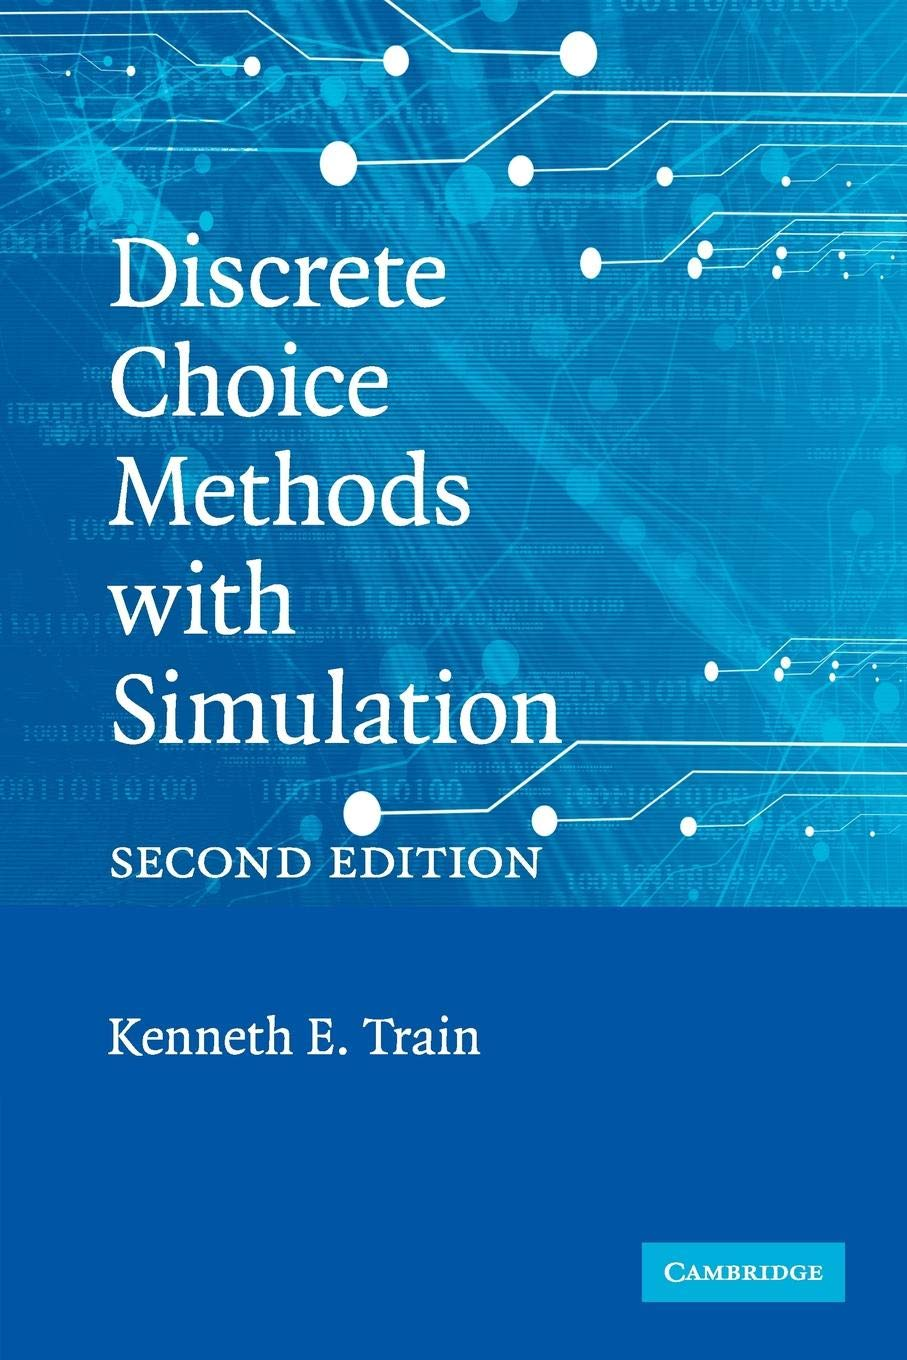
\includegraphics[width=0.2\linewidth]{train}
        \end{tabular} & 
        \begin{tabular}{l}
            \parbox{0.65\linewidth}{
            \emph{Discrete Choice Methods with Simulation\\ (Second Edition)}\\ Kenneth E.\ Train
            \begin{itemize}
                \item Available for free at: \href{https://eml.berkeley.edu/books/choice2.html}{\texttt{eml.berkeley.edu/books/choice2.html}}
                \item Paperback copy is usually less than $\$50$
            \end{itemize}
            }
        \end{tabular}
    \end{tabular} \\
    \vspace{3ex}
    \begin{itemize}
        \item I will also post supplemental notes on some topics that we cover
    \end{itemize}
\end{frame}

\begin{frame}\frametitle{Other References}
    \begin{tabular}{cl}  
        \begin{tabular}{c}
            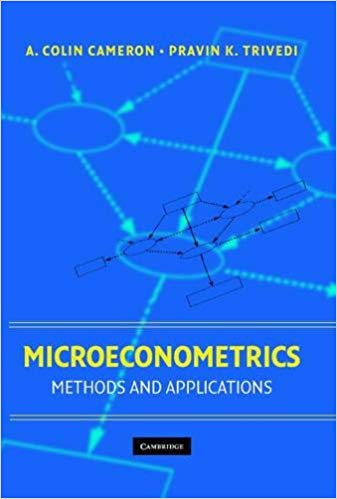
\includegraphics[width=0.1\linewidth]{cameron}
        \end{tabular} & 
        \begin{tabular}{l}
            \parbox{0.75\linewidth}{
            \emph{Microeconometrics:\ Methods and Applications}\\ A. Colin Cameron and Pravin K. Trivedi
            }
        \end{tabular}
    \end{tabular} \\
    \vspace{1ex}
    \begin{tabular}{cl}  
        \begin{tabular}{c}
            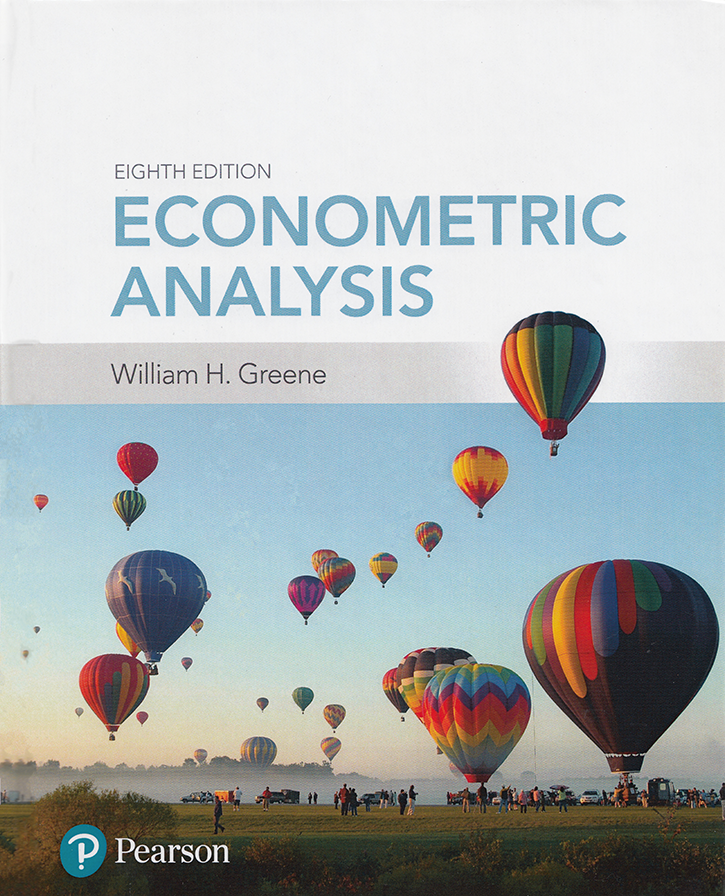
\includegraphics[width=0.1\linewidth]{greene}
        \end{tabular} & 
        \begin{tabular}{l}
            \parbox{0.75\linewidth}{
            \emph{Econometric Analysis}\\ William H. Greene
            }
        \end{tabular}
    \end{tabular} \\
    \vspace{1ex}
    \begin{tabular}{cl}  
        \begin{tabular}{c}
            
\includegraphics[width=0.1\linewidth]{hayashi}
        \end{tabular} & 
        \begin{tabular}{l}
            \parbox{0.75\linewidth}{
            \emph{Econometrics}\\ Fumio Hayashi
            }
        \end{tabular}
    \end{tabular} \\
    \vspace{1ex}
    \begin{tabular}{cl}  
        \begin{tabular}{c}
            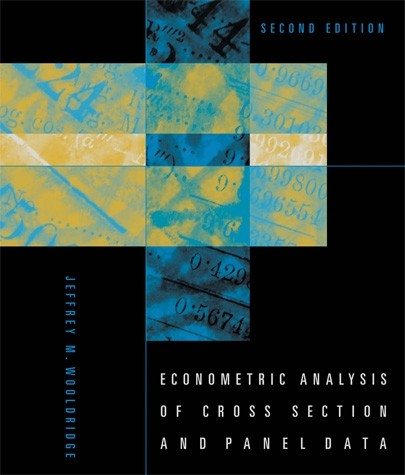
\includegraphics[width=0.1\linewidth]{wooldridge}
        \end{tabular} & 
        \begin{tabular}{l}
            \parbox{0.75\linewidth}{
            \emph{Econometric Analysis of Cross Section and Panel Data}\\ Jeffrey M. Wooldridge
            }
        \end{tabular}
    \end{tabular}
\end{frame}

\begin{frame}\frametitle{Software}
    We will use the R statistical programming language in this course \\
    \vspace{2ex}
    But I already know Stata/Matlab/Python/SAS/Julia. Why R?
    \begin{itemize}
        \item R is free and open source
        \item R is powerful and flexible
        \begin{itemize}
            \item Basic statistics, data cleaning, linear regression, matrix algebra, simulation methods, structural estimation, data visualization, etc.
        \end{itemize}
        \item R is favored by employers
    \end{itemize}
    \vspace{2ex}
    How can I learn R?
    \begin{itemize}
        \item R tutorial in Week 2
        \item Many R resources available for free
        \item First problem set will be a (relatively) gentle introduction to R
    \end{itemize}
    \vspace{2ex}
    You do not have to use R. But I will not provide any support or partial credit for work done in other programming languages.
\end{frame}

\begin{frame}\frametitle{Installing R}
    Installing R is \emph{usually} straightforward \\
    \vspace{1ex}
    \begin{tabular}{@{\extracolsep{-2ex}} c l}
        \begin{tabular}{c}
            
\includegraphics[width=0.05\linewidth]{r}
        \end{tabular} & 
        \begin{tabular}{l}
            \parbox{0.9\linewidth}{
            \href{https://cran.r-project.org/}{Download (\texttt{cran.r-project.org})} and install R
            }
        \end{tabular}
    \end{tabular} \\
    \vspace{1ex}
    \begin{tabular}{@{\extracolsep{-2ex}} c l}
        \begin{tabular}{c}
            
\includegraphics[width=0.05\linewidth]{rstudio}
        \end{tabular} & 
        \begin{tabular}{l}
            \parbox{0.9\linewidth}{
            \href{https://www.rstudio.com/products/rstudio/download/}{Download (\texttt{www.rstudio.com/products/rstudio/download})}\\ and install RStudio Desktop (Open Source License)
            }
        \end{tabular}
    \end{tabular} \\
    \vspace{3ex}
    What is the difference between R and RStudio? \\
    \vspace{1ex}
    \begin{tabular}{@{\extracolsep{-2ex}} c l}
        \begin{tabular}{c}
            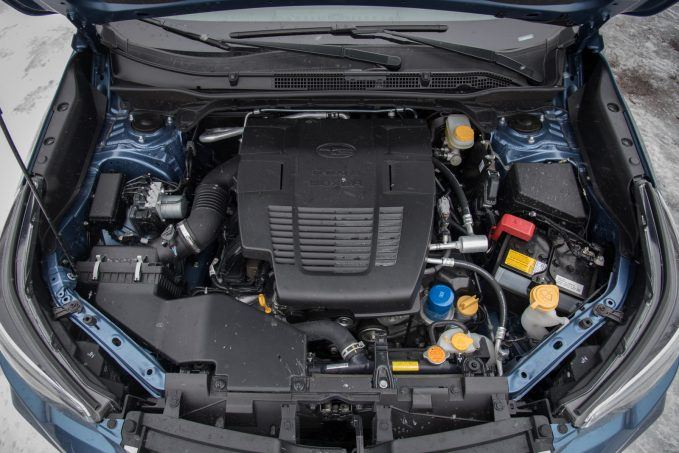
\includegraphics[width=0.25\linewidth]{engine}
        \end{tabular} & 
        \begin{tabular}{l}
            \parbox{0.65\linewidth}{
            R is like a car's engine. It is the program that powers your data analysis.
            }
        \end{tabular}
    \end{tabular} \\
    \vspace{1ex}
    \begin{tabular}{@{\extracolsep{-2ex}} c l}
        \begin{tabular}{c}
            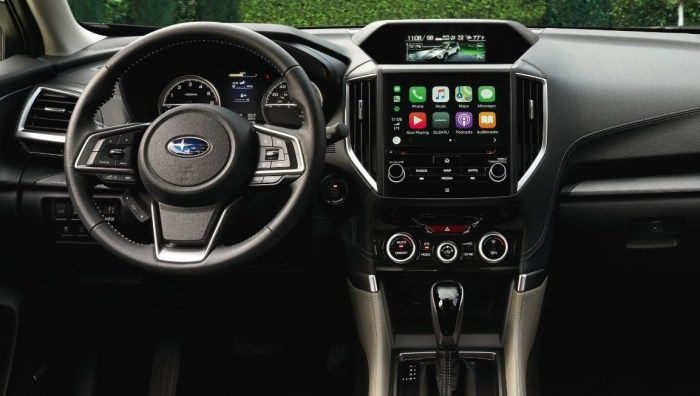
\includegraphics[width=0.25\linewidth]{dashboard}
        \end{tabular} & 
        \begin{tabular}{l}
            \parbox{0.65\linewidth}{
            RStudio is like a car's dashboard. It is the program you interact with to harness the power of your ``engine.''
            }
        \end{tabular}
    \end{tabular}
\end{frame}

\section{Grades and Assignments}
\label{grades}
\begin{frame}\frametitle{}
    \vfill
    \centering
    \begin{beamercolorbox}[center]{title}
        \Large Grades and Assignments
    \end{beamercolorbox}
    \vfill
\end{frame}

\begin{frame}\frametitle{Grades}
    Your final grade will be made up of
    \begin{itemize}
        \item Problem sets: 4 at 15\% each (60\% total)
        \item Final project: 30\%
        \item Participation: 10\%
    \end{itemize}
\end{frame}

\begin{frame}\frametitle{Problem Sets}
    Problems sets will simulate the kind of analysis you will do when conducting your own research
    \begin{itemize}
        \item Apply the estimation methods you learn in class
        \item Interpret your results
        \item Draw policy-relevant conclusions
    \end{itemize}
    \vspace{2ex}
    Rules for problem sets
    \begin{itemize}
        \item You can work in groups of up to three people (I recommend you do)
        \item Submit one write up with the names of all group members
        \item You must submit your code with your write up
        \item You can only use ``canned'' routines when told to do so
    \end{itemize}
    \vspace{2ex}
    See syllabus for tentative problem set schedule
\end{frame}

\begin{frame}\frametitle{Final Project}
    Final project will be similar to problem sets
    \begin{itemize}
        \item Estimation, interpretation, etc.
        \item At least ten days to complete
        \item Work in groups of up to three people
    \end{itemize}
    \vspace{2ex}
    How the final project differs from problem sets
    \begin{itemize}
        \item Closely mimics a real-world research project
        \item Will require roughly twice the effort of a problem set
    \end{itemize}
    \vspace{2ex}
    More details to come toward the end of the semester
\end{frame}

\begin{frame}\frametitle{Participation}
    In-person class attendance is not required but STRONGLY recommended when \emph{safely possible}
    \begin{itemize}
        \item You will be responsible for this material
        \item Classes will be recorded for later viewing
        \item If you miss a class, watch the recording (and sign up for office hours if helpful) to catch up on the material
    \end{itemize}
    \vspace{2ex}
    ``Participation'' is required
    \begin{itemize}
        \item Read the assigned reading
        \item Watch asynchronous lecture videos
        \item Keep up with in-class discussions and exercises
    \end{itemize}
    \vspace{2ex}
    See syllabus for tentative schedule of weekly topics and reading
\end{frame}

\end{document}